\documentclass{standalone}
\usepackage[T1]{fontenc}
\usepackage[latin2]{inputenc}
\usepackage[english]{babel}
\usepackage{tikz}
\usetikzlibrary{calc,through,backgrounds,positioning,fit}
\usetikzlibrary{shapes,arrows,shadows}
 
\begin{document}

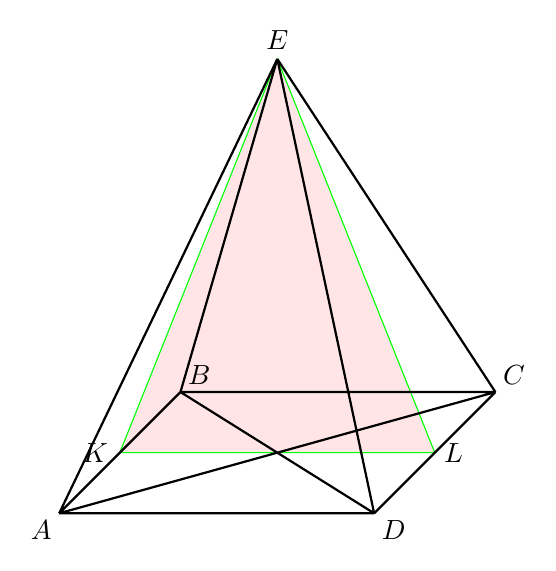
\begin{tikzpicture}[scale=1,inner sep=0.4mm]

\coordinate (A) at (0,0,4);
\coordinate (B) at (0,0,0);
\coordinate (C) at (4,0,0);
\coordinate (D) at (4,0,4);
\coordinate (E) at (2,5,2);
\coordinate (K) at (0,0,2);
\coordinate (L) at (4,0,2);

\filldraw [draw=green,fill=red!10]
	(K) -- (L) -- (E) -- cycle;

\draw [thick]	(A) -- (B)
	(B) -- (C)
	(C) -- (D)
	(D) -- (A)
	(D) -- (B)
	(A) -- (C)
	(E) -- (A)
	(E) -- (B)
	(E) -- (C)
	(E) -- (D);


\node at (A) [below left=2pt]{$A$};
\node at (B) [above right=2pt]{$B$};
\node at (C) [above right=2pt]{$C$};
\node at (D) [below right=2pt]{$D$};
\node at (E) [above=2pt]{$E$};
\node at (K) [left=3pt]{$K$};
\node at (L) [right=2pt]{$L$};


\end{tikzpicture}

\end{document}
